\chapter{Introduction}
Various defects in software can result from multiple developers working on the same code within a project \cite{livshits_01}.  Some errors introduced by the coding activities of developers may consist of behavioral differences within and between components and their interfaces \cite{leveson_01,smidts_01,nakajo_01}.  Other errors stem from inadequate comprehension of project code, supported by the fact that developers spend 50\% to 80\% of their time understanding it \cite{sinha_01}.  Furthermore, these kinds of misunderstandings can lead to bug fixes that inject more faults into code \cite{smidts_01}.

\indent
Comprehensive requirements analysis, design, and other good software development practices can prevent many post-delivery software problems \cite{boehm_01}, but cannot completely eliminate the possibility of human error.  Even well designed projects can get mired in code implementation details that hinder or prevent developers from delivering on time and within budget.

\indent
Code generation tools can improve the software development process by generating well-organized code reducing implementation errors and inconsistencies \cite{boysen_01}.  Code generation has been shown to improve the productivity of developers, guarantee correctness of syntax, and decrease errors \cite{groher_01}.  A compiler is a type of code generation tool that generates binary executables from code written in higher-level programming languages like C and C++.   Some tools generate higher-level code instead of binary given a set of rules known as a grammar.  This high-level generated code is then fed to a compiler to create a binary executable.

\indent
Most high-level code generation tools are specialized and only generate one part of an application’s overall implementation.  Popular targets for specialized code generation are lexical analyzers and parsers.  One of the earliest code generation tools is the compiler-compiler (parser generator), a term first presented in the early 1960’s \cite{brooker_01}.

\indent
The Yacc (“Yet Another Compiler Compiler”) \cite{johnson_01} compiler-compiler is a popular tool that generates parsers given (1) a context-free grammar to describe input, (2) an action (code snippets) to run for each token grouping that matches a grammar rule, and (3) code to provide input tokens to the parser.  This input specification is a hybrid between a declarative domain-specific language (i.e. a grammar) and an imperative programming language like C \cite{demetrescu_01,lloyd_01,gifford_01}.  Nevertheless, Yacc lacks the ability to read an input stream and convert it into tokens for parsing.

\indent
Lexical analyzer generators such as Lex and Flex must be used in conjunction with Yacc to accomplish this separate task of lexical analyzer generation \cite{johnson_01,lesk_01}.  The practice of using separate tools to generate a lexical analyzer and parser mean that input formats for each tool must be learned and used correctly to achieve the desired result.

\begin{figure}[htbp]
\centering
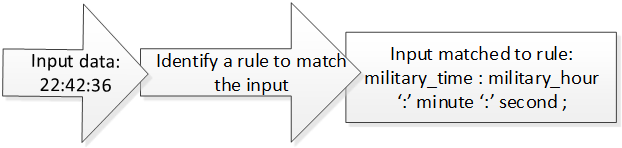
\includegraphics[width=0.9\textwidth]{figures/YaccGrammarRule.png}
\caption{Example Yacc grammar rule matched to input.}
\label{fig:YaccGrammarRule}
\end{figure}

\indent
Figure~\ref{fig:YaccGrammarRule} shows an example Yacc grammar rule matched to input formatted as military time.  In this example, military\_hour, minute, and second (all defined somewhere else in the grammar) describe specific parts of input data as military\_time.  When tokens match this rule, a code action is executed \cite{johnson_01,niemann_01}.

\indent
This report will present a new input specification based on Extended Backus-Naur Form (EBNF) called Typed-EBNF (TEBNF) (see appendix A), and a new prototype code generation tool that uses TEBNF as its input specification.  The tool will validate key features of TEBNF:
\begin{enumerate}
  \item TEBNF grammars can describe input patterns that include a mixture of strings, numbers, and/or raw groupings of bytes.
  \item TEBNF integrates grammar rules with states and actions.
  \item TEBNF can specify different methods of receiving input and sending output.
  \item TEBNF can declare how raw input data should be unmarshaled into well-known types of specific sizes (in bytes).
  \item TEBNF can declare how well-known types should be marshaled back into their original format.
  \item TEBNF provides typed and non-typed EBNF terminals.
  \item TEBNF supports arithmetic and non-arithmetic operations inside grammar rules.
  \item TEBNF grammars match specific pieces of a given input to well-known types of varied sizes (in bits or bytes).
  \item TEBNF supports the use of variables.
  \item TEBNF is Turing complete (see appendix B).
\end{enumerate}

\indent
The prototype code generation tool will demonstrate that it can generate a console application that can:
\begin{enumerate}
  \item Parse data from different kinds of inputs.
  \item Process data to produce specific output(s).
  \item Direct output(s) to a network destination (UDP/IP), a file, or a console-based user-interface.
  \item Support custom network protocol handling and interaction (UDP/IP).
  \item Provide a console-based user interface for the application. 
\end{enumerate}
